Das ALICE Experiment wurde speziell zur Untersuchung des Quark-Gluonen-Plasmas konzipiert und gebaut.
Um die Anspr\"uche daf\"ur besonders gut erf\"ullen zu k\"onnen besteht das ALICE Experiment aus einer Vielzahl unterschiedlicher Detektoren.
\begin{figure}[thp]
\centering
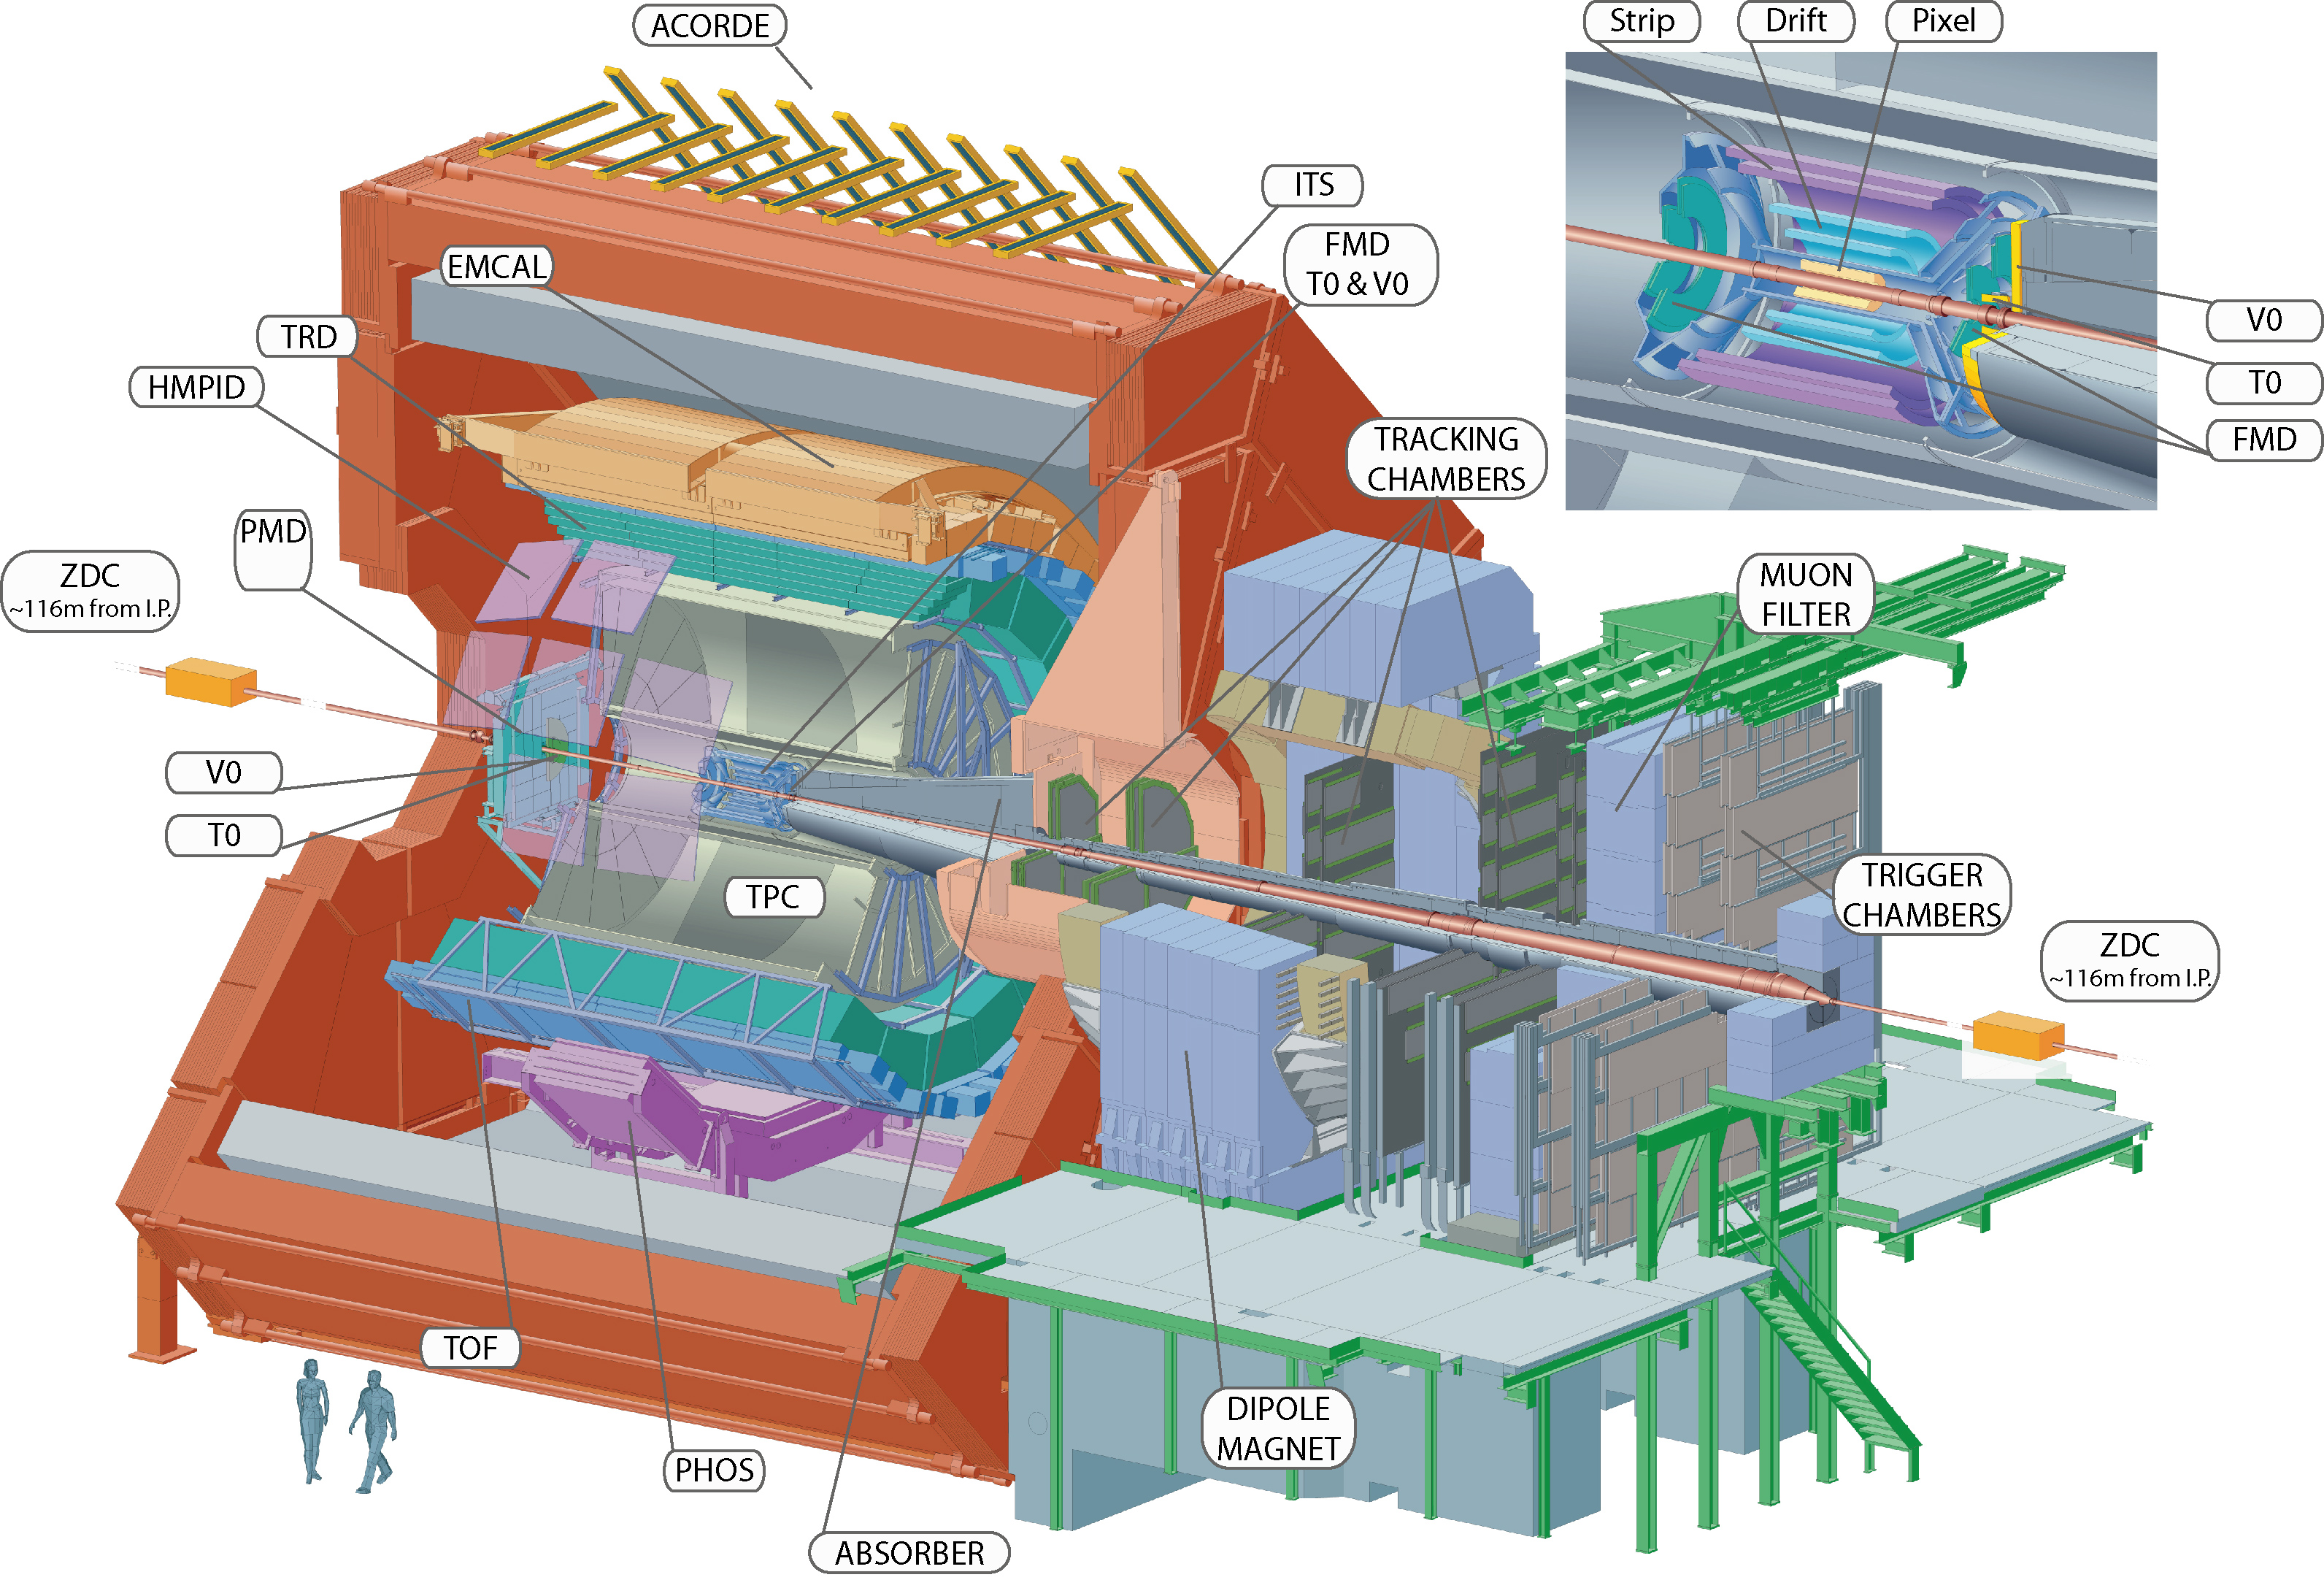
\includegraphics[width=.9\linewidth]{ALICE.jpg}
\caption{Schematische Darstellung des Querschnitts des ALICE Experiments.
\cite{WEBSITE:1}}
\label{fig:ALICE}
\end{figure}
Abbildung \ref{fig:ALICE} zeigt schematisch einen Querschnitt des ALICE Experiments. Der zylinderf\"ormige Aufbau um das Kollisionszentrum ist typisch f\"ur Kollisionsexperimente.
\newline
Um die zentralen Detektoren befindet sich ein gro{\ss}er roter Solenoid-Magnet, der ein Magnetfeld von 0,5 T erzeugt, wodurch geladene Teilchen auf gekr\"ummte Flugbahnen gelenkt werden.
Mit Hilfe der Radien k\"onnen einige der geladenen Teilchen identifiziert werden.
Im Folgenden werden die f\"ur diese Analyse wichtigsten Detektoren kurz eingef\"uhrt.
\newline
\textbf{Inner Tracking System}
\newline
Das Inner Trackign System, kurz ITS, befindet sich im innersten des ALICE Experiments und besteht aus sechs Schichten.
Von innen nach au{\ss}en au{\ss}en sind die Schichten zwei Silicon Pixel Detectors, kurz SPD, zwei Silicon Drift Detectors, kurz SDD, und zwei Silicon Strip Detectors, kurz SSD.
Das ITS wird haupts\"achlich zur Ortsbestimmung des sogenannten prim\"aren Vertex benutzt.
Der prim\"are Vertex ist die Absch\"atzung des Kollisionspunktes.
\newline
\textbf{Time Projection Chamber}
\newline
Die Time Projection Chamber, kurz TPC, umschlie{\ss}t das ITS und dient als zylinderf\"ormiger Detektor der Spurrekonstruktion.
Die TPC ist mit Gas gef\"ullt und hat an beiden Enden jeweils eine Hochspannungselektrode, wodurch zwei gegens\"atzliche elektrische Felder im inneren der TPC vorliegen.
Fliegen geladene Teilchen durch die TPC, so ionisieren die geladenen Teilchen das Gas.
Das ionisierte Gas wiederum wird durch das elektrische Feld in Richtung der Endplatten beschleunigt, an denen sich auch Ausleseelektronik befindet.
Durch die Bahnkr\"ummung, sowie der Dichte der Gasionisation von den geladenen Teilchen k\"onnen die geladenen Teilchen identifiziert werden. \cite{PAPER:2}
\newline
\textbf{V0-Detektoren}
\newline
Die sogenannte V0-Detektoren bestehen aus zwei einzelnen Detektoren, welche sich jeweils an einem Ende des ITS um die Strahlenachse befinden.
Messen beide V0 Detektoren eine bestimmte Mindestanzahl an Teilchen, so wird die Aufzeichnung einer Kollision (engl. \textit{Event}) gestartet.
Solche Anforderungen werden allgemein als \textit{trigger} bezeichnet, diese Anforderung, dass die V0-Detektoren eine Mindestanzahl an Teilchen detektieren m\"ussen, nennt man entsprechend \textit{minimum-bias trigger}.
\newline
\textbf{T0-Detekroren}
\newline
Genauso wie die V0-Detekroren bestehen die T0-Detektoren auch aus zwei einzelnen Detektoren, welche sich ebenfalls an den Enden der ITS befinden.
Bei den T0-Detektoren handelt es sich um pr\"azise Zeitdetektoren, die der genauen Bestimmung des Kollisionszeitpunkts dienen.
\newline
\textbf{Elektromagnetische Kaloriemeter}
\newline
Das elektromagnetische Kaloriemeter, kurz EMCal, befindet sich am \"au{\ss}ersten Rand des zentralen Detektorkomplexes.
Aufgrund der Wichtigkeit des EMCals f\"ur diese Analyse wird das EMCal im folgenden Abschnitt genauer erl\"autert.